\subsection{Формула Тейлора}
Пусть функция \( n \) раз дифференцируема. \\
Рассмотрим формулу дифференцируемой функции:
\[ f(x) = f(x_0) + f'(x_0)(x-x_0) + o(x-x_0) \]
Рассмотрим бесконечно малую функцию \( o(x-x_0) \):
\[ o(x-x_0) = c_2(x-x_0)^2 + o_2(x-x_0), c_2 \in \R \]
%% Добавить иллюстрацию 1 - images/1.jpg (jpg -> tikz)
\begin{figure} 
    \centering
    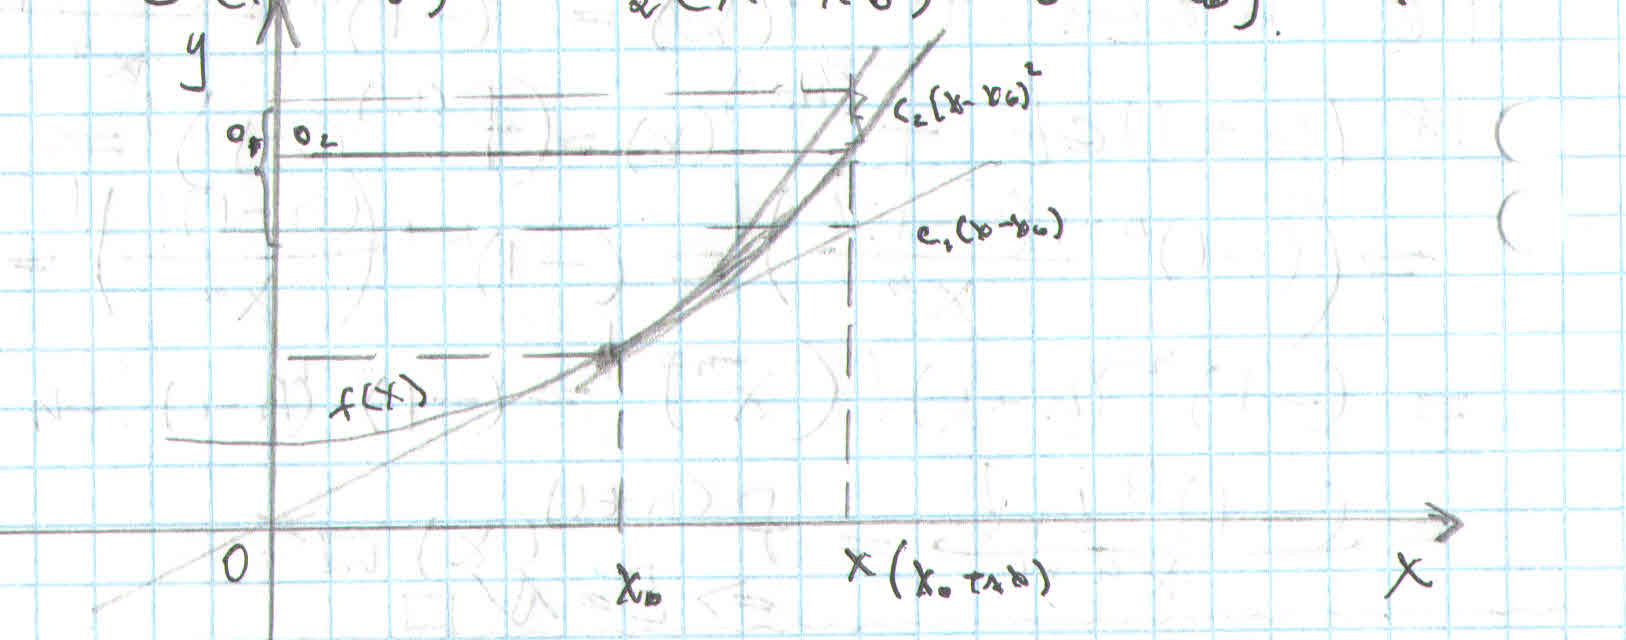
\includegraphics[width=0.5\textwidth]{1}
    \caption{\label{fig:diffGeom} Приближение при помощи дифференциалов}
\end{figure} \\ 
Продолжая так раскрывать все последующие б.м.ф., мы получим следующую картину:
\[ f(x) = c_1(x-x_0)+c_2(x-x_0)^2+\dots+c_n(x-x_0)^n+R_n(x) \]
Остаётся узнать, какие коэффициенты \( c_{1}, \dots, c_{n} \) нужно подставить. \\ 
\[ c_k = \frac{f^{(k)}(x_0)}{k!} \text{-- коэффициенты Тейлора} \]
Пусть \( P(x) \) -- полином: 
\[ P(x) = \mum{i=1}{n}{c_i(x-x_0)^i} \]
Тогда \( R_n(x) \)(остаток Тейлора) будет равен \( 0 \).
\[ P(x_0) = f(x_0) \]
\[ P'(x_0) = c_1 \Longrightarrow c_1 = \frac{P'(x_0)}{1!} \]
\[ P''(x_0) = 2c_2 \Longrightarrow c_2 = \frac{P''(x_0)}{2!} \]
\[ P'''(x_0) = 6c_3 \Longrightarrow c_3 = \frac{P'''(x_0)}{3!} \]
Таким образом, \[ c_k = \frac{P^{(k)}(x_0)}{k!} \]
Рассмотрим функцию \( f \). Коэффициенты будем строить так же: \( c_k  = \frac{f^{(k)}(x_0)}{k!}\) -- построим полином \( T_n \) (многочлен Тейлора) для \( n \) раз дифференцируемой функции:
\[ T_n(x) = \mum{k=0}{n}{\frac{f^{(k)}(x_0)}{k!}(x-x_0)^k} \]
Но \( T_n \) и \( f \) в общем случае не совпадают - нам нужно добавить \( R_n \) -- остаточный член формулы Тейлора (остаток формулы Тейлора).
\begin{note} 
    Если \( x_0 = 0 \), то мы получим формулу Маклорена: %%% РЯД? у нас же здесь получается частичная сумма! (?)
    \[ f(x) = \mum{k=0}{n}{\frac{f^{(k)}(0)}{k!}x^k} + R_n(x) \]
    % Вот же ряд: 
    % \[ f(x) = \mum{k=0}{+\infty}{\frac{f^{(k)}(x)}{k!}x^k} \]
    % У нас тогда должно быть следующее необходимое условие существования ряда: функция должна быть бесконечно раз дифференцируема в окрестности 0
\end{note}